%included in thesis.tex,



\chapter{Background and Literature Study}
This chapter will try to outline the basics needed to understand this report. Mathematical
knowledge are crucial to understand the principles used in robot navigation and decision
making. The topics treated here include, general reference frames, homogeneous coordinate
representations, camera modeling, feature matching, map representations and optimization
criterions.



\section{Basics}

\subsection{Reference Frames}
	Movement must be described relative to something. This is the task of the reference systems. There are
	4 important reference system. The ECI (Earth Centre Inertial) which is a truly inertial reference
	frame, i.e. it is not accelerating. Its axis are pointing through the north pole and through the
	equatorial line of the Earth, fixed toward stationary points in space. The centre is as the name
	suggests in the centre of the Earth. 
	
	ECEF (Earth-Centre Earth-Fixed) is another reference frame. It is defined same as the ECI coordinate
	system, but the axis are rotating with the same rate as the Earths rotation rate. This means that this frame
	is not
	strictly inertial, but the angular velocity of the Earths rotation are considered very small, and can
	be neglected compared to other velocities in the same frame. Position on the earth are described by
	\emph{longitude} and \emph{latitude}.

	An important reference frame when considering local motion are the NED (North East Down) frame. This
	frame is defined as the tangent plane on the current position, and moving with the object. The axis
	are pointing towards north, east and down. This frame can be used in local, and small areas, but are
	not valid for intercontinental travel. This frame will primarily be used in this report. 

	The last but important frame are the Body frame, which is the local frame of the object of interest.
	The body frame are defined as the x-axis along its forward movement, y-axis to the right of the
	movement direction, and the last pointing downward, to complete the right-hand system. The
	origin are defined in the Centre of Gravity of the object. This frame are convenient when
	defining velocities, forces and moments. More on reference frames in \cite{fossen} and
    \cite{forsell}.
    \begin{figure}[htbp]
        \centering
       % \includegraphics[width=0.7\textwidth]{pics/referenceframse}
        \caption{The different reference frames in this report}
        \label{chap2:fig-ref-frames}
    \end{figure}

    The reference frames that will be considered in this report are the \emph{NED}- and
    \emph{body} frames. In addition to these two frames there are the last, but not least
    important frame, called the \emph{single-sensor} frame. This is where the output from
    the sensors are defined. These output need to be transformed into the \emph{body} and
    to the \emph{NED} frame to make sense for the control system and ultimately for the
    user. 

    The \emph{single-sensor} frames are where the individual sensors give readings. The
    exact mount point relative to the centre-of-gravity need to be defined, to make the
    transformation to other frames possible. The domain of the \emph{single-sensor} frames
    are defined in accordance to the domain of the sensor, i.e. the domain of a Laser
    Range Finder, which gives angles and ranges in the plane are two dimensional. 

    \begin{figure}[htbp]
        \centering
        %\includegraphics[width=0.7\textwidth]{pics/singlesensorframes}
        \caption{\emph{Single-Sensor} frames on PiKo}
        \label{chap2:fig-single-sensor-frames}
    \end{figure}


\subsection{Homogeneous Transformation Coordinates}
To represent transformations, i.e. rotations, translations, shear and scaling, it is
practical to represent those transformations in matrix form. But it is not mathematically
possible to represent both rotations and translations in the same matrix as long as it is
contained in $\mathbb{R}^3$. ******REFERENCE******

To overcome this problem, the coordinates are projected into a fourth dimensional space.
All points and vectors gain an extra element which describes if the coordinate is a vector
or a point. 
\begin{equation}
        \mathbf{v} = \left[ \begin{array}{c}
                                    x_v \\
                                    y_v \\
                                    z_v \\
                                    w_v  \end{array} \right]  =
                     \left[ \begin{array}{c}
                                    1 \\
                                    0 \\
                                    0 \\
                                    0  \end{array} \right] \quad \quad
        \mathbf{p} = \left[ \begin{array}{c}
                                    x_p \\
                                    y_p \\
                                    z_p \\
                                    w_p  \end{array} \right]  =
                     \left[ \begin{array}{c}
                                    1 \\
                                    0 \\
                                    0 \\
                                    1  \end{array} \right] \quad \quad
\end{equation}
Here $\mathbf{v}$ is a vector with the fourth element as zero, while $\mathbf{p}$ is a
point with the fourth element equal one.

This leads us to the \emph{Transformation Matrix} which is a $4 \times 4$ matrix. For
example a matrix representing rotation and translation will look like this
\begin{equation}
    \label{chap2:eq-TransformationMatrix}
    \mathbf{T_{rt}} = \left [ \begin{array}{cccc}
                                r_{xx} & r_{xy} & r_{xz} & t_x \\
                                r_{yx} & r_{yy} & r_{yz} & t_y \\
                                r_{zx} & r_{zy} & r_{zz} & t_z \\
                                0  & 0  & 0  & 1  \end{array} \right]
\end{equation}
Here the $r_{ii}$ coefficients are rotation parameters and the $t_i$ coefficients are the
translation parameters. The rotation coefficients are calculated from the Euler angles.

Likewise, scaling might be performed by the following transformation matrix
\begin{equation}
    \label{chap2:eq-TransformationMatrixScaling}
    \mathbf{T_S} = \left [ \begin{array}{cccc}
                                S_x & 0 & 0 & 0 \\
                                0 & S_y & 0 & 0 \\
                                0 & 0 & S_z & 0 \\
                                0 & 0 & 0 & 1 
                                 \end{array} \right]
\end{equation}
All of this transformations might be combined into a single matrix by multiplying the
matrices together, in the reverse of the order of which the transformations are carried
out. 


\section{Ranging Techniques}
The measure of distances and ranges are important and there are various ways of doing
this. Most techniques include the measure of time-of-flight of some signal and calculating
the distance from the known travel velocity of the signal. This requires the signal
emitted to be reflected, captured and processed at or close to the emitter. The signal is
usually electromagnetic or sound based, which allows for different kinds of modulations to
make the signal easier to recognize at the receiver.


This section will first outline the usual range determination techniques then go into the
more specific sensor characteristics in later sections.


\subsection{Triangulation}
The technique of triangulation is an old and well-known technique for range determination.
Two points with known locations are used. The distance between the two points are called
the \emph{baseline}. Instead of measuring the range to a third point directly the angles
from the two ends of the baseline to a third point is used to calculate the range
according to Equation \ref{chap2:eq-triangulation}. See Figure
\ref{chap2:fig-triangulation}.
\begin{equation}
    \label{chap2:eq-triangulation}
    d = b \frac{\sin{\alpha} \sin{\beta}}{\sin{\alpha + \beta}}
\end{equation}
\begin{figure}[htbp]
    \caption{Triangulation setup}
    \label{chap2:fig-triangulation}
\end{figure}

This technique is accurate for as long as all the points are in the same plane.


\subsection{Time-of-Flight Measurement}
This method of range determination is the most common, and utilizes the travel time of the
emitted signal. The signal might be in light, radio or sound waves. The precision of the
range greatly depend on the type of signal, the medium which it travels and the quality of
the time-measuring device. By knowing the velocity of the emitted signal and assuming it
is constant, the distance it travels can be determined with great accuracy according to 
Equation \eqref{chap2:eq-tof}
\begin{equation}
    \label{chap2:eq-tof}
    d = v \frac{t}{2}
\end{equation}



\section{Various Sensors Used in Robotics}
This section concerns the use of different kind of sensors in robotic applications. Only
sensors which are compliant to the overall perspective will be dealt with. This includes
laser range finders, ultrasound and Sonar sensors, Time-of-Flight cameras and
stereo cameras. 

\subsection{2D Sensors}

\subsubsection{Laser Range Finders}


When looking at Laser Range Finder, there are 3 techniques for determining the distance,
\emph{optical triangulation}, \emph{pulse Time-of-Flight} and \emph{frequency modulated
continuous wave} (FMCW). \cite{laser-ranging-critical-review}

\paragraph{Optical Triangulation}
Optical is very similar to triangulation described above and uses the same principle.
A light source are placed at the one end of the
baseline, and a light sensor at the other end which senses the reflected light from the
light source. The principle is basically the same as in normal triangulation. But, due to
the fact that a light source is used, and more closely a laser light source, the surface
that the laser light hits, the dot detected by the photo detector at the other end of the
baseline, needs to ''stay in focus``. If this is not done the laser dot will become a
blurred disc and the uncertainty to the point will become larger. To force the dot to
always be in focus, a special aligning of the lenses and photo detector are used, called 
the \emph{Scheimpflug} condition. The interested reader are referred to
\cite{laser-ranging-critical-review}.

The laser dot is contaminated with speckle noise which makes it more difficult to find the
exact center of the projected dot. This makes the determination of the along the third
dimension a bit more tricky, because of the positional uncertainty introduced by the
noise. Frequency of the light, angle and area of the collecting lenses and photo detector
are parameters that influence the position uncertainty. 


\paragraph{Pulsed Time-of-Flight}
The technique referred to as pulsed time-of-flight refers to the time taken of a pulse
train of laser light to be reflected back to the emitter. Light travels around $30$cm/ns,
this means that to get $1$mm accuracy the accuracy of the timing devices should be
$6.7$ps.

The application and ranges that are going to be measured are dependant on what kind of
laser which is selected. The energy in the laser pulse effects the amplitude of the
reflected light and in turn affects the measurement accuracy.



\paragraph{Frequency Modulated Continuous Wave}




\subsubsection{Sonar}


\subsubsection{Infrared Sensors and Proximity Sensors}


\subsection{3D Sensors}


\subsubsection{Time-of-Flight Cameras}
The research and application of Time-of-Flight cameras have increased significantly during the last four
years. A Time-of-Flight camera is a compact device which makes it suitable to mount on
mobile platforms, and thereby using it in navigation and localization applications. 

The most used ranging techniques by the cameras are \emph{intensity modulation} approaches and
\emph{optical shutter} technology. The first one is used by the best known manufacturers,
like MESA and PMD. While the optical shutter approach is less expensive and have been used
by Zcam, which now have been sold to Microsoft. 


\paragraph{Intensity Modulation Approach}
This approach uses modulated near infrared light (NIR), $g$ which is reflected to and
captured by a CCD chip then correlated with the reference signal, $r$. 
\begin{equation}
    c(\tau) = g \otimes r = \lim_{T \rightarrow \inf} \int^{T/2}_{-T/2} g(t) r(t + \tau) dt
\end{equation}
where the signals, $g$ and $r$ might be
\begin{equation}
    g(t) = \cos{\omega t}, \quad \quad r(t) = b + a \cos{(\omega t + \phi)}
\end{equation}
where $\phi$ is the phase offset because of the travel time of the signal, $b$ is a
correlation bias, $a$ is the amplitude and $\omega$ is the modulation frequency. Solving
the integral yields 
\begin{equation}
    c(\tau) = \frac{a}{2} \cos{(\omega \tau + \phi )} + b
\end{equation}
which is the correlation function. 

The demodulation is usually done by sampling the correlation function at 4 equally spaced
phase offsets. The following relation can now be written
\begin{equation}
    \begin{aligned}
        \phi &= \tan^{-1} (\frac{A_3 - A_1}{A_0 - A_2}) \\
        I &= \frac{A_0 + A_1 + A_2 + A_3}{4} \\
        a &= \frac{\sqrt{(A_3 - A_1)^2 + (A_0 - A_2)^2}}{2}
    \end{aligned}
\end{equation}
where $A_i = c(i \frac{\pi}{2})$ for $ i = 0,..,3$ and $I$ is the intensity of the returned NIR
signal. From this the distance can be calculated using the phase delay $\phi$. 
\begin{equation}
    d = \frac{c}{4 \pi \omega} \phi
\end{equation}

There are a number of challenges when using this approach
\cite{time-of-flight-comp-graphics}
\begin{itemize}
    \item The resolution of the sensors are small compared to standard RGB or grayscale
        sensors. Current resolution on present day time-of-flight cameras are $204 \times
        204$. 
    \item ``Wiggling'' because of imperfections when creating the sinusoidal signals.
    \item Errors due to intensity measurements. Various sensor electronics might influence
        the measured intensity and give wrong readings.
    \item ``Flying Pixels'' occurs when a pixel in the camera oversees a region with
        large depth variances, e.g. at object boundaries, because of superimposed signals. 
    \item Motion artifacts might occur because the phase images are captured sequentially
        quick motion might cause artifacts.
    \item Multiple reflections in highly reflective environments will cause erroneous
        distance measurements.
\end{itemize}

Standard lenses are used to capture the reflected light, which means that intrinsic
calibration should be carried out to specify the projection axis and distortion parameters
of the lens. See sections below for lens calibration and distortion coefficient
estimation. \cite{time-of-flight-comp-graphics}


\paragraph{Optical Shutter Approaches}
Light travels roughly at $c \approx 3 \times 10^8$ meters per seconds. This translates to
that light uses $7$ pico seconds to travel one millimeter. Imagine a light pulse emitted
at time $t$. This pulse travels in a spherical pattern and hits a 3D shape. The light wall
will be reflected back in a distorted pattern.\cite{optical-shutter} 
A shutter in front of the CCD chip then
shuts out the rest of the light wall pattern. This will then produce a shape of the object
which can be used to calculate the distance, based on the times the shutter is open,
according to the following relation \cite{time-of-flight-comp-graphics}
\begin{equation}
    d = (1 - \alpha) d_{min} + \alpha d_{max}, \quad \quad \alpha =
    \frac{I_{gate}}{I_{total}}
\end{equation}
where $I_{gate}$ is the pixel intensity which arrives when the shutter is open, and
$I_{total}$ is the total amount of reflected light. Distances outside $d_{min}$ and
$d_{max}$ cannot be measured in the exposure. Therefor this techniques require multiple
exposure to get the desired depth resolution. 

This method is also prone to the challenges stated for the intensity modulation approach
as well. 



\subsubsection{Stereo Vision}
Stereo vision is an inexpensive way of finding range measurements. The setup is two or
more cameras some distance away from each other. This distance is called the
\emph{baseline}. The camera images are then compared and a common reference point is
found. The difference between the images are then used together with the baseline distance
to triangulate the common reference point and then find the distance to the observed
object. 

The process of Stereo Imaging involves 4 steps when using two cameras \cite{openCV}:
\begin{enumerate}
    \item Remove radial and tangential lens distortion caused by inexpensive lenses and
        image chips. This outputs \emph{undistorted} images. 
    \item \emph{Rectify} the images. This adjusts the angles and distances between the cameras.
        This outputs row-aligned images.
    \item Find the same features in the left and right camera view. This process is called
        finding \emph{stereo correspondences}. This outputs a \emph{disparity} map, which
        is the difference in x-coordinate of the feature in the left and the right image. 
    \item If the geometric configuration of the cameras are known, the disparity map can
        be translated into depth map with the help of \emph{triangulation}. This final
        step is called \emph{reprojection}.
\end{enumerate}
This steps will be described in detail below. 


\paragraph{Pinhole Camera Model}
A camera model is needed to understand how light is captured on the image plane. To do
this a \emph{pinhole camera} model is used to capture light form a point. This model
assumes that only one light ray from each point travels trough a infinite small hole in
a plane, called the \emph{focal} plane and hits a second plane, called \emph{image} plane.
These two planes are placed a distance, $f$ from each other. Using elemental geometry the
coordinates of the real world point imaged at the image plane can be calculated. 
\begin{equation}
    -x_i = f \frac{X}{Z}
\end{equation}
where
\begin{equation}
    P_i = \left [ \begin{array}{c}
        x_i \\
        y_i 
    \end{array} \right]  \in \mathbb{R}^2 \quad \quad P_w = \left [
    \begin{array}{c}
        X \\
        Y \\
        Z \\ 
    \end{array} \right] \in \mathbb{R}^3 
\end{equation}
\begin{figure}[hbtp]
    \centering
    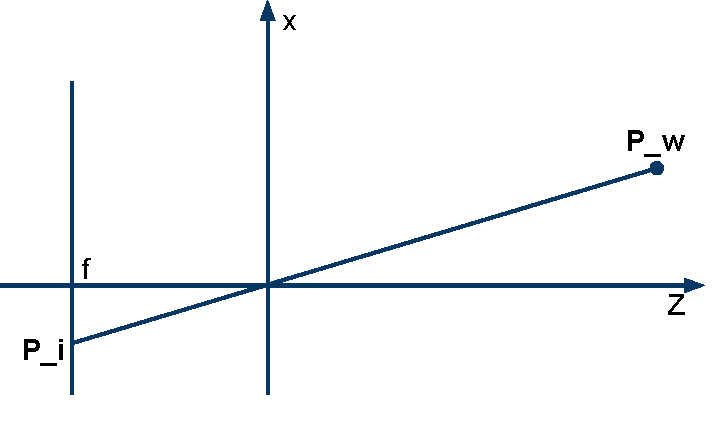
\includegraphics[width=0.7\textwidth]{pics/pinhole_model}
    \caption{Pinhole Camera Model showing two dimensions}
    \label{fig:ch2-pinhole}
\end{figure}

Figure \ref{chap2:fig-pinhole} shows the configuration with the pinhole located at
Origo and the image plane located at $f$. Where the pinhole is are often termed
\emph{center of projection}. The x axis of the image is located
upwards, while the real Z axis are the horizontal axis, that are called the
\emph{optcal axis}. This lead us to the next parameters which need to be defined.

The optical axis should ideally always be aligned with the center of projection. Due to
manufacturing inaccuracies this is rarely the case, therefor we need two more parameters
in to complete the pinhole model equations. This parameters are $c_x$ and $c_y$ which
describes the offset of the optical axis from the center of projection. Also the need for
different focal lengths in $x$ and $y$ might also be a necessity, because the individual
pixels on a typical low-cost image chip is rectangular rather than square. Now the
equations relating real-world coordinates to image coordinates can be written.
\cite{openCV}
\begin{equation}
    x_i = f_x \frac{X}{Z} + c_x \quad \quad y_i = f_y \frac{Y}{Z} + c_y
\end{equation}

The equations above are the \emph{projective} transformations, and are convenient to
write using homogeneous coordinates and arrange the parameters into a single $3\times 3$
matrix. This matrix is sometimes called the \emph{camera intrinsic} matrix. 

\paragraph{Lens Distortion}
Because very little light goes through the pinhole, and to make the camera practical for
real world use, lenses are used to bend, i.e. focus more light to the projective plane.
This allows for faster imaging of the world, but is also the source of more distortions
and inaccuracies. 

There are two types of lens distortions, \emph{radial} and \emph{tangential}. Radial
distortions are due to the lens construction. Most distortion occurs towards the edges of
the lens. This can be seen in pictures as ``barrel'' or ``fish-eye'' effects. These
effects are more present in cheap cameras which does not have the fancy lenses and optics
that the more high-end cameras have. There is also other types of distortions in imaging
systems, but they have typical lesser effects on the images, and will not be taken into
account. 

To model radial lens distortions the approach described by Brown in
\cite{lens-calibration} are used. The radial distortion are in practice small and can be
described by the two first terms of a Taylor series expansion around the center of the
lens. If the lens have high radial distortion, like fish-eye lenses a third term are
appended. The radial location of the point on the image plane can in general be described
like the equations below. 
\begin{equation}
\begin{aligned}
    x_{corrected} &= x_i ( 1 + k_1 r^2 + k_2 r^4 + k_3 r^6 ) \\
    y_{corrected} &= y_i ( 1 + k_1 r^2 + k_2 r^4 + k_3 r^6 ) 
\end{aligned}
\end{equation}

Tangential distortion is due to manufacturing defects which causes the lens not to be
perfectly parallel to the imaging plane. This causes the image to become more like a
trapezoid. This can be modeled by equations \eqref{chap2:eq-tangential-distortion}. The
derivation of this equations can be found in \cite{brown66}.
\begin{equation}
    \label{chap2:eq-tangential-distortion}
    \begin{aligned}
        x_{corrected} &= x_i + (2 p_1 y_i + p_2 (r^2 + 2 x_i^2)) \\
        y_{corrected} &= y_i + ( p_1 (r^2 + 2 y_i^2) + 2 p_2 x_i))
    \end{aligned}
\end{equation}
The parameters $p_1$ and $p_2$ are the tangential distortion parameters. This parameters
gives enough information about the lens and camera to make corrections to the picture and
make the matching method easier and the measurements more accurate. This calibrations will
be shown in Chapter \ref{chap3-sensors} for the selected stereo cameras. 


\paragraph{Epipolar Geometry}
To describe the stereo rig and geometry between the left and right cameras, the term
\emph{epipolar geometry} is introduced. Epipolar geometry exists between any two cameras.
The different center of projections, $O_r$ and $O_l$, and corresponding
projective planes, $\Pi_r$ and $\Pi_l$ and the term \emph{epipole} on the projective plane
$\Pi_r$, $e_r$ can now be defined as the image of the center of projection of the other 
camera, $O_l$. Suppose the point, $P$ are viewed from both cameras, and have the image
location, $p_l$ and $p_r$ in the left and right view, respectively. The line from the left
epipole, $e_l$ to $p_l$ and the line from $e_r$ to $p_r$ are called the \emph{epipolar
lines}. The planes made by the observed real world point, $P$ and the center of
projections, $O_r$ and $O_l$ are called the \emph{epipolar planes}. See Figure
\ref{chap2:fig-epipolarGeometry}
\begin{figure}[htbp]
    \centering
    %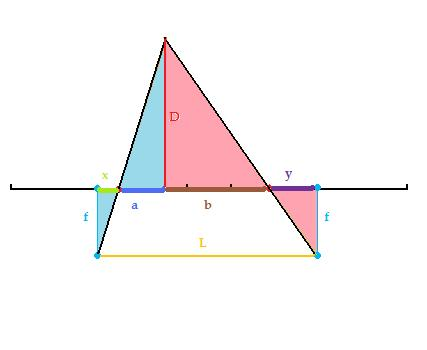
\includegraphics[width=0.5\textwidth]{pics/stereo_geometry}
    \caption{The epipolar geometry}
    \label{chap2:fig-epipolarGeometry}
\end{figure}

This allows for the following facts which simplifies the computations a great deal.
\cite{epipolar}
\begin{itemize}
    \item Every 3D point in view of the cameras is constrained in an epipolar plane that
        intersects each image in an epipolar line.
    \item The \emph{epipolar constraint} says that a given feature in one image must lie
        along the corresponding epipolar line in the other view.
    \item The epipolar constraint means that the two-dimensional search for matching
        features simplifies to a one-dimensional search along the epipolar lines once the
        epipolar geometry of the stereo rig is known.
    \item The order is preserved. If two points are visible in both images and occur
        horizontally in that order in one image, they occur in the same order in the other
        image.
\end{itemize}

\paragraph{The Essential and Fundamental Matrices}
This matrices contains information about the translation and rotation which relate the
two cameras. The Essential matrix describes this translation and rotation in physical
space, while the Fundamental matrix also contains information about the intrinsics of the
two cameras, thereby describing the rotations and translations in pixel related
coordinates.

The derivation of the Essential matrix is interesting and is given here for reference.
Suppose a point $P$ related in the left camera coordinates, i.e. $P_l$ and the right
camera is located at $T$. The coordinates of $P_l$ in the right camera coordinates will
then be.
\begin{equation}
    \label{chap2:eq-Pr}
    P_r = R (P_l - T)
\end{equation}
Now, the epipolar plane is introduced. All points, $\mathbf{x}$ that lay on the plane with normal vector
$\mathbf{n}$ and passing through $\mathbf{a}$ obeys the equation,
\begin{equation*}
    (\mathbf{x} - \mathbf{a}) \cdot \mathbf{n} = 0
\end{equation*}
The cross product of $T$ and $P_l$ then becomes the normal vector of the epipolar plane,
because the epipolar plane includes both this vectors. Equation \eqref{chap2:eq-Pr} can be
rewritten as $P_l - T = R^{-1} P_r$ and including the cross product yields 
\begin{equation}
    (R^{-1} P_r)^T (T \times P_l) = 0
\end{equation}
The cross product can be expressed as a product between matrices by introducing the
skew-symmetric matrix $S$. \cite{modsim}
\begin{equation}
    S = \left [ \begin{array}{ccc}
                0 & -T_z & T_y \\
                T_z & 0 & -T_x \\
                -T_y & T_x & 0 \\ \end{array} \right]
\end{equation}
The essential matrix might now be defined with $R^{-1} = R^T$ and moving it behind $P_r$.
\begin{equation}
    E = RS 
\end{equation}
which gives the equation
\begin{equation}
    \label{chap2:eq-fundamental}
    P_r^T E P_l = 0
\end{equation}
$P_r$ and $P_l$ are the real world 3D coordinates, and can be transformed to 2D
coordinates by the perspective transformation derived by the pinhole camera model. 

The relation between the Essential matrix and the Fundamental matrix can be showed with
help of the camera intrinsic matrix $M$, because we know that $q = Mp$, where $q$ are
pixel coordinates and $p$ are the 2D world coordinates. Substituting for $P$ in Eqauation
\eqref{chap2:eq-fundamental} gives: \cite{openCV}
\begin{equation}
    q_r^T(M_r^{-1})^T E M_l^{-1} q_l = 0
\end{equation}
The definition of the fundamental matrix, $F$ is then
\begin{equation}
    F = (M_r^{-1})^T E M_l^{-1}
\end{equation}
Both matrices are $3\times3$ and have rank two with seven parameters.


\paragraph{Finding Stereo Correspondences}
Now that the mathematics which describes points in the different views to each other, the
case of matching the same points together can begin. This is obviously only possible for
visual areas that the two camera views overlap. 

There are couple of different matching algorithms. The most common are \emph{block
matching} algorithms. In \cite{konolige} a practical implementation of the block
matching algorithm are described. This algorithms use sum of absolute difference (SAD) windows to match same
same points in the two views. This algorithm work only on undistorted, rectified stereo
images. It first normalizes the image brightness which enhances textures. Then the search
for correspondences are carried out along the horizontal epipolar lines using the sum of
absolute difference window. After this the results are filtered to eliminate bad stereo
matches. This algorithm works best in highly textured environments, like outdoor
environments, and will prove less effective in structured surroundings like office
corridors and inside smooth pipelines. 

Another common matching algorithm are \emph{graph cut} algorithms. 

An extensive review of the different matching algorithms and their computational costs
can be seen in \cite{stereo-algorithms}.


\paragraph{Disparity and depth calculations}
When finally the stereo correspondences are found, the \emph{disparity} can be calculated.
The disparity is the difference in pixels coordinates from of the matched feature from one
image to the other. This disparity is inversely proportional to the depth. This means that
the depth perception of the stereo rig is better when relatively close to the cameras, as
Figure \ref{chap2:fig-disparity-depth} shows.
\begin{figure}[htbp]
    \centering
    %\includegraphics[width=0.5\textwidth]{pics/disparity-depth}
    \caption{The relationship between depth and disparity}
    \label{chap2:fig-disparity-depth}
\end{figure}

Many robotic applications using stereo cameras utilizes the disparity maps directly,
because they usually just require the detection of obstacles. ****REFERENCES ON THIS****

The 3D coordinates of the point can be calculated form the disparities given by the
matching algorithms. This is the process of \emph{reprojection}. Using triangulation
between the two known camera locations the depth can be derived accordingly to 
\begin{equation}
    D = f (T / d - 1)
\end{equation}

\begin{figure}[htbp]
    \centering
    %\includegraphics[width=0.5\textwidth]{pics/stereo-triangulation}
    \caption{Triangulation in the stereo rig}
    \label{chap2:fig-stereo-triangulation}
\end{figure}




\section{Map Data Representation}
The representation of sensor data is important for the functionality of the robot. This is
dependant on the amount of processing power and capacity that is available at the robot.
The area which the robot is to map is also of great importance when choosing the
representation. There are a number of representations that are tried out, and each one has its good and
bad abilities. 

The major representation methods which is used in literature are summarized in the below
sections. There are two major ideas when it comes to map representation, and that is
metric and topological.

Metric representation uses the sensor data as we see it. It is the direct Cartesian
representation of the way the world is. Examples of this are CAD drawings of floor plans
and housing. This maps are often large and inexact, because of many kinds of
uncertainties.

Topological representations uses a more abstract way. The world are represented by graphs,
which is nodes and links between them. This are a sparse and efficient way of representing
the world, but need more processing when the map is built. This kind of maps are not
exact, because they are not expected to be. They simply describe the connection between
different kind of objects, and all objects might have attributes describing how it really
looks. This method is useful in highly structured environments, such as pipelines, sewers,
and office landscapes. This because a series of junctions might tell you where you are
than just the metric information, which might be quite erroneous. 


\subsection{Occupancy Grid Maps}
Occupancy grid maps are a metric approach to the mapping problem and are widely used in 
robotic mapping, mostly because of it is simple to implement and use. It was developed 
by Elfes and Moravec in the mid 1980s, \cite{elfes}, \cite{moravec}. The method is quite 
robust and it is simple to implement with many kinds of sensors. This method assumes that 
the robots pose is known.

This method divides the world into grids with probabilities that the grid is occupied. It
starts with all grids at 50 \%, equal probability that the space is occupied or not. As
the robot moves around it updates the grids according to its sensor readings. When for
example employing laser range finders, the grid at the distance reported from the range
finder are marked as occupied according to some uncertainty set by the accuracy of the
range finder. The grids between the possible detected obstacle will then be decreased
because the probability of obstacles are less. 

Occupancy maps are not the most computationally effective way to represent the world,
especially when it is big. It is cumbersome and may lead to problems when dealing with
cyclic environments. This because of the uncertainty in the sensor measurements and robots
pose and odometry. 


\subsection{Quad- and Oct-trees}
Quadtrees can be used to represent a 2D space by recursively dividing the space into
exactly four rectangles or squares. If this rectangles or squares does not include
interesting information then it will not be divided further. This dividing continues until
the smallest possible square is achieved. This creates a tree structure which is easily
traversed and searched if necessary. 

\begin{figure}[htbp]
    \centering
   %\includegraphics[width=0.5\textwidth]{pics/quad-tree}
    \caption{A Quadtree representation}
    \label{chap2:fig-quadtree}
\end{figure}


\subsection{Topological Maps}
Object maps are topological maps and represents the sensed world in the form of predefined nodes and links
between them. Each node has a set of attributes, like length, links to doors etc. This is
a compact way to express the world and is much more computationally effective with larger
maps than the occupancy grid maps might be. Examples of such nodes are corridors,
junctions and dead ends, but this nodes must be suited to the application of the robot. 

The problem with this representation is that it needs a lot of input \'a priori. The
operator creates and inputs the map to the robot, which uses this map for navigation. The
largest challenge with this is to make the robot aware of where it is. It needs in some
way to recognize its surroundings, and match it to the \'a priori map.


\subsection{Mixed Approaches}
This is when you take the best of both worlds. The easy and effective way of the metric
maps, and mix them with the abstract topological maps. This will help reduce the size of
the maps in the robots memory, and also make it more computationally effective because the
maps are sparse. 

******?????The mixed approaches are usually not computed on-line***???? (CHECK THIS). This utilizes
the metric approach for the rooms that have a lot of details, chairs, desks etc. and for
corridors and less detailed areas the topological approach, when the metric and
geographical information are not that important. 

This requires lots of processing of the sensor and map data, and should be done off-line
after the robot's mission is finished. 


\section{Sensor Fusion Techniques}
According to \cite{sensor-fusion-mobile-robots} theres a lot of ways to achieve sensor
fusion in mobile robotics. The use of multiple sensors are favorable because the readings
can be fused to make a better estimate of the current situation. 

Multi sensor fusion are widely used in robotics today. This because it allows the designer
to use different measurement principles which have different capabilities. 


\begin{itemize}
    \item Low-level Fusion with unknown statistics
        \begin{itemize}
            \item Rule-based
            \item Geometric and topological maps
        \end{itemize}
    \item Low-level Fusion with known statistics in centralized approaches
        \begin{itemize}
            \item Kalman Filter and probabilistic approaches
        \end{itemize}
    \item Low-level fusion with known statistics in decentralized architectures
        \begin{itemize}
            \item Decentralized probabilistic approaches
        \end{itemize}
    \item High-level Fusion
        \begin{itemize}
            \item Behaviour-based architectures
        \end{itemize}
\end{itemize}


\subsection{Low-level Fusion}
The term low-level fusion is often used when the sensor data is directly integrated
resulting in parameters and state estimates of the model. This methods are mostly purely
mathematical. This method involves the Kalman Filter, and other Bayesian approaches. In
many cases the use of \'a priori information are utilized to verify or improve the
estimates from the sensors.

This methods are probabilistic and requires that you know something about the
statistical properties of the sensors and the \'a priori model. 


\subsection{High-level Fusion}



\subsection{Interpolation Techniques}



\subsection{Probabilistic Techniques}



\section{Feature Extraction}
The need for feature extraction should be obvious when dealing with autonomous robot
navigation. For the robot to know where it is it needs to recognize its surroundings. This
is a difficult step, because computers are not known to be very good at this, as the human
brain is. 

By feature extraction it is meant to recognize one point or feature in one instant and
find the same point at the next time instant. This can be imagined difficult in some
surroundings where theres little individual detail. 

This problem is relaxed a bit when the surroundings are confined to pipelines. The problem
here is that the interior of the pipeline are not rich in detail, and is mostly the same
everywhere the robot travels, except in the different kinds of junctions. By feature
extraction in this report the meaning is to recognize the different types of junctions
that the robot will travel through. 
\cite{theilemann-breivik}



\subsection{Surface Fit Algorithms}


\subsubsection{Gauss-Newton Optimization}


\subsubsection{RANSAC Algorithm}


\subsubsection{M-SAC Criterion}



\section{Real World Applications}

Remember MAKRO! The German snake robot used for sewer inspections. 



